\documentclass[12pt,onecolumn]{IEEEtran}

% center captions
\makeatletter
\long\def\@makecaption#1#2{\ifx\@captype\@IEEEtablestring%
\footnotesize\begin{center}{\normalfont\footnotesize #1}\\
{\normalfont\footnotesize\scshape #2}\end{center}%
\@IEEEtablecaptionsepspace
\else
\@IEEEfigurecaptionsepspace
\setbox\@tempboxa\hbox{\normalfont\footnotesize {#1.}~~ #2}%
\ifdim \wd\@tempboxa >\hsize%
\setbox\@tempboxa\hbox{\normalfont\footnotesize {#1.}~~ }%
\parbox[t]{\hsize}{\normalfont\footnotesize \noindent\unhbox\@tempboxa#2}%
\else
\hbox to\hsize{\normalfont\footnotesize\hfil\box\@tempboxa\hfil}\fi\fi}
\makeatother

\usepackage{mathtools}
\usepackage{bm}
\usepackage{graphicx}

\usepackage[nospace]{cite}
\bibliographystyle{IEEEtran}

\usepackage{MnSymbol}
\usepackage{listings}
\lstset{
  basicstyle=\ttfamily,
  numbers=left,
  numberstyle=\small,
  stepnumber=1,
  frame=single,
  breaklines=true, prebreak=\raisebox{0ex}[0ex][0ex]{\ensuremath{\rhookswarrow}}, postbreak=\raisebox{0ex}[0ex][0ex]{\ensuremath{\rcurvearrowse\space}},
  %moredelim=**[is][\btHL]{@}{@},
}

\title{ECE 6604 Design Project:\\ Performance of STBC Schemes over Rayleigh Block-Fading Channel for 4G MIMO}
\author{Abhishek~Obla~Hema and~Klaus~Okkelberg}

\newcommand*\dif{\mathop{}\!\mathrm{d}}
\newcommand{\trans}{^\text{T}}
\newcommand{\herm}{^\text{H}}
\newcommand{\order}[1]{\mathcal{O}(#1)}
\DeclareMathOperator{\E}{E}
\DeclareMathOperator{\trace}{trace}

\begin{document}

\maketitle

\begin{abstract}
  Wireless mobile networks are a part of everyday life, but they have limited range and data rate to satisfy the demands of the exponentially increasing number of wireless mobile devices. In particular, high energy consumption and spectrum contraints mean that current 3.9G technology will not be able to satisfy the demands of mobile data traffic in the near future. To overcome these limitations, various diversity schemes are used, which fall into six categories, namely time, space, angle, polarization, frequency, and multipath. One implementation of a diversity scheme is to use MIMO links, which use multiple transmit and receive antennas to increase time and spatial diversity, the result of which is to increase range and data rate without requiring additional transmit power or bandwidth. To this end, this paper investigates the performance of space-time block coding (STBC) schemes for up to eight transmit antennas and up to two receive antennas, in line with current 4G standards for cellular phones. These schemes are analyzed for their spectral efficiency and bit error rates for transmitting data modulated using BPSK, QPSK, 16-QAM, and 64-QAM over a Rayleigh block-fading channel with additive white Gaussian noise. This is accomplished through software simulation in Matlab.
\end{abstract}

\section{Introduction}
%%% Local Variables:
%%% mode: latex
%%% TeX-master: "report"
%%% End:

% Section I: Introduction

Current wireless high-speed data communication standards are considered to be 3.9G with 4G technologies deploying in the near future. Of the 3.9G technologies, Long Term Evolution (LTE) developed by the 3rd Generation Partnership Project (3GPP) is far more popular than IEEE 802.16e WiMAX. LTE is commonly marketed as 4G LTE even though it does not comply with ITU-R IMT-Advanced requirements to be considered 4G. Current 4G standards include 3GPP Long Term Evolution Advanced (LTE-A) and IEEE 802.16m WiMAX Release 2, with LTE-A being the more popular of the two currently. This delay in the development and deployment of actual 4G standards means that future 5G standards have a lot of catching up to do in order to meet the exponentially increasing number of mobile devices, each with greater data needs. To this end, this paper explores one possible method of meeting those needs, namely using massive MIMO systems with appropriately chosen space-time block codes.

The paper is organized as follows. The remainder of this section discusses the motivation and implementation of LTE and LTE-A. Section II provides background on diversity-increasing schemes used in current 3.9G and 4G standards, especially MIMO. Section III discusses current STBC schemes. Section IV explains the simulation methodology. The simulation results are presented and analyzed in section V. Finally, section VI summarizes the results and discusses how they can be applied to future 5G technologies. The simulation code used for this paper is included in the appendix.

\subsection{LTE}

LTE is a registered trademark owned by ETSI (European Telecommunications Standards Institute) for the wireless data communications technology and a development of the GSM/UMTS standards. LTE is based on the GSM/EDGE and UMTS/HSPA network technologies, increasing the capacity and speed using a different radio interface together with core network improvements. LTE is the natural upgrade path for carriers with both GSM/UMTS networks and CDMA2000 networks. The different LTE frequencies and bands used in different countries mean that only multi-band phones are be able to use LTE in all countries where it is supported.

The goal of LTE was to increase the capacity and speed of wireless data networks using new digital signal processing (DSP) techniques and modulations that were developed around the turn of the millennium. A further goal was the redesign and simplification of the network architecture to an IP-based system with significantly reduced transfer latency compared to the 3G architecture. The LTE wireless interface is incompatible with 2G and 3G networks, so it must be operated on a separate radio spectrum. The LTE specification provides downlink peak rates of 300~Mbit/s, uplink peak rates of 75~Mbit/s and QoS provisions permitting a transfer latency of less than 5ms in the radio access network. LTE has the ability to manage fast-moving mobiles and supports multi-cast and broadcast streams. LTE supports scalable carrier bandwidths, from 1.4~MHz to 20~MHz and supports both frequency division duplexing (FDD) and time-division duplexing (TDD). The IP-based network architecture, called the Evolved Packet Core (EPC) designed to replace the GPRS Core Network, supports seamless handovers for both voice and data to cell towers with older network technology such as GSM, UMTS and CDMA2000. The simpler architecture results in lower operating costs (for example, each E-UTRA cell will support up to four times the data and voice capacity supported by HSPA)

LTE supports deployment on different frequency bandwidths. The current specification outlines the following bandwidth blocks: 1.4MHz, 3MHz, 5MHz, 10MHz, 15MHz, and 20MHz. Frequency bandwidth blocks are essentially the amount of space a network operator dedicates to a network. Depending on the type of LTE being deployed, these bandwidths have slightly different meaning in terms of capacity. That will be covered later, though. An operator may choose to deploy LTE in a smaller bandwidth and grow it to a larger one as it transitions subscribers off of its legacy networks (GSM, CDMA, etc.).

LTE uses two different types of air interfaces (radio links), one for downlink (from tower to device), and one for uplink (from device to tower). By using different types of interfaces for the downlink and uplink, LTE utilizes the optimal way to do wireless connections both ways, which makes a better-optimized network and better battery life on LTE devices.

For the downlink, LTE uses an orthogonal frequency division multiple access (OFDMA) air interface as opposed to the code division multiple access (CDMA) and time division multiple access (TDMA) air interfaces . OFDMA (unlike CDMA and TDMA) mandates that multiple-input, multiple-output (MIMO) is used. Having MIMO means that devices have multiple connections to a single cell, which increases the stability of the connection and reduces latency tremendously. It also increases the total throughput of a connection. MIMO is what lets 802.11n WiFi reach speeds of up to 600Mbps, though most advertise up to 300-400Mbps. There is a significant disadvantage though. MIMO works better the further apart the individual carrier antennae are, in order to increase spatial diversity. On smaller phones, the interference caused by the antennae being so close to each other will cause LTE performance to drop. 

For the uplink (from device to tower), LTE uses the  discrete Fourier transform spread OFDMA (DFTS-OFDMA) scheme of generating a single carrier frequency division multiple access (SC-FDMA) signal. As opposed to regular OFDMA, SC-FDMA is better for uplink because it has a better peak-to-average power ratio over OFDMA for uplink. LTE-enabled devices, in order to conserve battery life, typically do not have a strong and powerful signal going back to the tower, so a lot of the benefits of normal OFDMA would be lost with a weak signal. Despite the name, SC-FDMA is still a MIMO system. LTE uses a SC-FDMA $1\times2$ configuration, which means that for every one antenna on the transmitting device, there are two antennae on the base station for receiving.

The LTE technology itself also comes in two flavors: an FDD (frequency division duplex) variant and a TDD (time division duplex) variant. The most common variant being used is the FDD variant. The FDD variant uses separate frequencies for downlink and uplink in the form of a band pair. That means for every band that a phone supports, it actually uses two frequency ranges. These are known as paired frequency bands. For example, Verizon’s 10MHz network is in FDD, so the bandwidth is allocated for uplink and downlink. This is commonly noted as a 2x10MHz or 10+10 MHz configuration. Some also call it 10x10MHz, but this is mathematically incorrect, but they mean 10+10MHz. Some will also call it a 20MHz network, but this can be ambiguous. The TDD variant uses one single range of frequencies in a frequency band, but that band is segmented to support transmit and receive signals in a single frequency range.

For example, an LTE TDD network deployed on 20MHz of spectrum uses the whole chunk as one large block for frequency allocation purposes. For network bandwidth purposes, a LTE TDD network’s spectrum can be further divided to optimize for the type of network traffic (half up and half down, mostly down and a bit up, mostly up and a bit down, and so on).

\subsection{LTE-A}

LTE-A is a major enhancement of the LTE standard that meets 4G requirements. It was standarized by 3GPP as 3GPP Release 10. Presently, there are few deployments and almost no capable smartphones.

The main developments of LTE-A over LTE are~\cite{TR36_912}
\begin{itemize}
\item Ability to use up to $8\times8$ MIMO and 128-QAM in downlink
\item Up to 100~MHz of carrier aggregated bandwidth
\item Higher spectral efficiency with a maximum of 30~bps/Hz in LTE-A release 10 versus 16~bps/Hz in release 8
\item 1~Gbit/s peak data rate per user
\item Increased peak data rate of 3~Gbit/s download and 1.5~Gbit/s upload
\item Faster switching between power states
\item Improved performance at cell edges
\end{itemize}
Even with these enhancements, LTE-A is backwards compatible with LTE, meaning an LTE mobile station would work in an LTE-A network and vice versa.

\subsection{Impact of LTE on Battery Life}

By itself, LTE devices should last roughly as long as their HSPA+ equivalents because of the optimized radios for both downlink and uplink operations. The reason why LTE devices right now eat batteries for breakfast is because the network operators are forcing many of these devices into active dual-mode operation.

For Verizon Wireless, this means that most of their LTE devices connect to both CDMA2000 and LTE simultaneously and stay connected to both. This consumes twice the amount of battery for every minute connected than if the phone were connected only to CDMA2000 or LTE. Additionally, when calls are made on Verizon Wireless LTE phones, the CDMA2000 radio sucks down more power because you are talking. Sending and receiving text messages causes pulses of CDMA2000 activity, which cuts battery life more. Arguably, constantly changing radio states could be worse for battery life than a switch into one mode for a period of time and switching back, so text messages may actually kill the batteries faster.

Also of importance for battery life is handover. Handover is the operation in which a device switches from one network to another or from one tower to another. Handover is the critical component that makes any cellular wireless network possible. Without handover, a user would have to manually select a new tower every time the user leaves the range of a tower. For cellular networks, this is even more critical because the range of a tower is not very predictable due to factors outside of anyone’s control (like the weather, etc.). LTE supports handover like all other cellular wireless networks, but it improves on it by doing it much faster when handing over to a supported type of network or cell.

\section{MIMO and Diversity}
% Section II: Background

MIMO: A General Overview
MIMO technology is one of the most important technologies to improve the system performance in capacity, coverage and the user data rates. The performance gains depend on the propagation characteristics of each scenario. Wi-Fi, LTE, and many other radio both RF as well as wireless technologies use the new MIMO wireless technology to increase the link capacity, spectral efficiency and the link reliability using interference paths.

A channel will be affected by fading and this will in turn have an adverse impact on the SNR. This will then impact the error rate, if the data transmitted is digital. Diversity is the principle in which we give the receiver multiple versions of the same signal. If they can be made to be affected in many ways by a signal path the probability that they will be affected at the same time is reduced. Hence we can see that diversity is crucial in improving the performance of the link, stabilizing it as well as reducing the error rate. 
There are several diversity modes that are available and provide a number of advantages. 

	Time diversity: In time diversity, a message is transmitted at different times, e.g. using different timeslots and channel coding. 

	Frequency diversity: In this form we use different frequencies. It may be in the form of using different channels, or technologies such as spread spectrum OFDM. 

	Space diversity: Space diversity is used as the basis for MIMO. It uses the antennas that are located in multiple positions to take advantage of the different radio paths that exist in a typical environment. 

Time diversity:
In this type of diversity we averaging the fading of the channel over time by using the channel coding and interleaving to let every part of the code word affected by different fading along the time so if a deep fading occurs only part of the code word will being missing not all the code word to explain this we will see an example:















Frequency diversity:
	Frequency hop spread-spectrum:
Frequency hopping is one of two basic modulation techniques used in spread spectrum signal transmission. It is the repeated switching of frequencies during radio transmission, often to minimize the effectiveness of "electronic warfare" - that is, the unauthorized interception or jamming of telecommunications. It also is known as frequency- hopping code division multiple access (FH-CDMA).
In an FH-CDMA system, a transmitter "hops" between available frequencies according to a specified algorithm, which can be either random or preplanned. The transmitter operates in synchronization with a receiver, which remains tuned to the same center frequency as the transmitter. A short burst of data is transmitted on a narrowband. Then, the transmitter tunes to another frequency and transmits again. The receiver thus is capable of hopping its frequency over a given bandwidth several times a second, transmitting on one frequency for a certain period of time, then hopping to another frequency and transmitting again. Frequency hopping requires a much wider bandwidth than is needed to transmit the same information using only one carrier frequency.

	Direct sequence spread-spectrum
In direct sequence spread spectrum, the stream of information to be transmitted is divided into small pieces, each of which is allocated across to a frequency channel across the spectrum. A data signal at the point of transmission is combined with a higher data-rate bit sequence (also known as a chipping code) that divides the data according to a spreading ratio. The redundant chipping code helps the signal resist interference and also enables the original data to be recovered if data bits are damaged during transmission.
In general, frequency-hopping devices use less power and are cheaper, but the performance of DS-CDMA systems is usually better and more reliable.
      

Spatial (antenna) diversity:
In this type of diversity we assures that we will have many copies of the transmitted signal or a coded versions effects with different fading over the space as we use multi antenna systems at the transmitter or the receiver to have finally at the receiver many copies of the transmitted signal suffers from different fading and the type of the diversity defined by where the multi antenna system so we have this types of the spatial diversity.


MIMO is a radio antenna technology as it uses multiple antennas placed at the transmitter as well as receiver so that a variety of signals carry data through different paths and we choose the separate paths for each antenna so that the multiple paths can be used.

















                                                      Figure 8. MIMO System

It is found that in between a transmitter and receiver, the signal can travel through multiple paths. So moving the antennas by even a small amount will lead to a change. The different number of paths that are available occurs as a result of a number of objects that appear in the direct path between the transmitter and receiver. Before these paths were just used to introduce interference but now using MIMO they can be used as an advantage. The two main formats of MIMO are: 

	Spatial diversity: This refers to transmit and receive diversity. They provide improvement in the SNR and are characterized by boosting the reliability of the system with respect to fading. 

	Spatial multiplexing: This provides additional data capacity by using the different paths to carry traffic, thereby increasing the total throughput of the system. 

Since we use multiple antennas, MIMO can increase the capacity of a channel and still obey Shannon’s Law. With every pair of antennas that are added to the network, it is possible to linearly boost the throughput by increasing the receive and transmit antennas. Since the spectrum bandwidth is a very valuable commodity, such techniques are necessary to use the bandwidth that is available more efficiently and MIMO is one of those valuable techniques.

There are a number of MIMO configurations or formats that have been used. Each format has its own advantages and disadvantages and they can be used and balanced to provide the optimum solution for a particular application. The different MIMO formats – SISO, SIMO, MISO, MIMO all require different number of antennas and each requires different complexity. Depending on the format post processing might be required at one end or the other.

The different forms of antenna technology refer to the single or multiple inputs or outputs which are related to the radio link. In this way the input is the transmitter as it transmits into the system and the output is receiver.



The different forms of single / multiple antenna links are defined as below:

	SISO - Single Input Single Output

	SIMO - Single Input Multiple output

	MISO - Multiple Input Single Output

	MIMO - Multiple Input multiple Output



 






































A. MIMO-SISO 


The simplest form of radio link is SISO- Single Input Single Output. In this the transmitter operates with one antenna with the receiver. In this scheme no diversity and no additional processing is required. This can be viewed from the first figure.

B. MIMO-SIMO

In this scheme the transmitter has a single antenna while the receiver has multiple ones. This is called as receiver diversity. This is used to support a receiver system that receives signals from a number of sources to counter the effects of fading. This scheme has been in use for a long time with short wave listening/ receiving stations to fight ionospheric fading and interference. This is represented by the second figure. The main advantage is that is easy to implement however some processing is required at the receiver side. The use of SIMO is widespread but the receiver is located as a handset, hence it may be limited by size, cost and drain. There are two forms of SIMO that can be used:

	Switched diversity SIMO: Here it finds the strongest signal and switches to antenna.

	Maximum ratio combining SIMO: It collects both the signals and combines them to give a combination. Hence the signal from both contributes to the total signal.

C. MIMO-MISO:

MISO is also called as transmit diversity, where the same data is transmitted repeatedly from two transmitters. The receiver can then extract the needed data from the optimum signal. This is represented by the third figure. The main advantage of this scheme is that the multiple antennas and the repeated coding/processing is shifted from the receiver to the transmitter. If we take the case of cellphones, this results in massive savings in terms of space and reduces the processing required for coding. Again this results in reduced batter consumption, costs and smaller size.

D. MIMO:

In this case there are multiple antennas at the transmitter as well as the receiver. It provides advantages in total channel throughput. This scheme has been represented by the fourth and final figure. This requires coding to separate the data from the multiple paths which requires processing but boosts the total throughput and capacity.

There are many types of MIMO that can be used from SISO, through SIMO and MISO to complete MIMO networks. These are all able to provide heavy gains in performance, but usually at the expense of processing and total number of antennas. Tradeoffs have to be made between cost, performance, size, battery life before we choose the correct scheme.

%%%%%%%%

Rayleigh fading of signals yields a very large performance loss by converting the exponential dependency of bit error probability $P_b$ on the mean received bit energy-to-noise ratio $E_b/N_0$ into an inverse linear one. Diversity is one remedy that improves the reliability of communication by providing the receiver with multiple independently-faded copies of the same information. These copies are often referred to as diversity branches. Diversity methods can be categorized as those that exploit (1) spatial, (2) angle, (3) polarization, (4) frequency, (5) multipath, and (6) time diversity. At the receiver, the diversity branches are combined together, with the most effective combining method depending, among other things, on the type of additive impairment. For additive white Gaussian noise (AWGN) dominant channels, maximal ratio combining (MRC) is optimal in the maximum likelihood (ML) sense. For co-channel interference (CCI) dominant channels, optimum combining performs better.

The performance of a diversity scheme is measured by its diversity gain, defined as the number of independent receptions of the same signal. The independent copies of the signal increase the signal-to-interference ratio and allow a reduction in transmission power without a performance loss. A MIMO system with $N_T$ transmit antennas and $N_R$ receive antennas has a maximum diversity gain equal to $N_TN_R$.


\section{Space-Time Block Coding}
%%% Local Variables:
%%% mode: latex
%%% TeX-master: "report"
%%% End:

% Section III: STBC

With the carrier frequencies used in current 3.9G and 4G standards, only up to two receive antennas can be used while maintaining spatial diversity. Thus, it is necessary to use transmitter diversity, which uses multiple transmit antennas to provide the receiver with multiple uncorrelated copies of the same signal. Simple forms of transmit diversity include selective transmit diversity for time division duplexed systems as well as time division transmit diversity, time-switched transmit diversity, and delay transmit diversity for frequency division duplexed systems. More complex forms of transmit diversity use space-time, space-frequency, or space-time-frequency coding.

For MIMO systems, knowledge of the channel state information (CSI) at the transmitter (CSIT) and at the receiver (CSIR) is necessary to choose a diversity technique~\cite{caire03,weingarten06}. In general, the channel can be estimated at the receiver using various techniques (see~\cite{nasseri10,bjornson10,biguesh06}), so the knowledge of the CSIR can be assumed. At the transmitter, if the CSIT is known, then beamforming techniques are used to assure both the diversity gain and the array gain. However, without CSIT, space-time (ST) codes can still be used to assure the diversity gain. ST codes are a general class of error correcting codes in which the control symbols are inserted in both spatial and temporal domains.

The multi-layered space-time architecture was introduced by Foschini in~\cite{foschini96}. Later, Space-Time Trellis Codes (STTrC)~\cite{tarokh98} were proposed, which provide the optimal tradeoff between constellation size, data rate, diversity gain, and trellis complexity but have a greater decoding complexity. Regarding encoding and decoding complexity, Alamouti~\cite{alamouti98} introduced a simple repetition diversity scheme for two transmit antennas with maximum likelihood combining at the receiver. Alamouti's transmit diversity scheme provides a maximum diversity gain and no coding gain for a minimum decoding complexity. Later, Tarokh et al.\ generalized the Alamouti code for an arbitrary number of transmit antennas as the Space-Time Block Code (STBC)~\cite{tarokh99}.

The remainder of this section presents a mathematical model for a general MIMO system using STBC and details ML decoding methods for both linear and widely linear coding schemes. Additionally, some examples of STBCs are reviewed with emphasis on the code transmission matrix and the code parameters.

\subsection{Space-Time Block Coded MIMO System}
This paper considers digital wireless transmissions through a general MIMO system with $N_T$ transmit antennas and $N_R$ receive antennas, consisting of a ST encoder, a Rayleigh block-fading channel with AWGN, and a ST decoder with MRC and ML decoding. The channel is modeled as a discrete-time baseband-equivalent channel. This study assumes single-carrier modulated block transmission with zero padding is used to suppress intersymbol interference (ISI) and prevent inter-channel interference (ICI), as in~\cite{wang00,wang04} and uncorrelated path gains for the receive antennas.

\subsubsection{Space-Time Encoding}
Assume that the input to the ST encoder is a $k$-dimensional vector of complex symbols $\bm{s}=[s_1\,s_2\,\cdots\,s_k]\trans$. The encoding method for the STBC is defined by its transmission matrix in the form 
\[ \bm{G} = \begin{bmatrix}
  g_{11} & g_{12} & \cdots & g_{1N_T} \\
  g_{21} & g_{22} & \cdots & g_{2N_T} \\
  \vdots & \vdots &       & \vdots \\
  g_{T1} & g_{T2} & \cdots & g_{TN_T}
\end{bmatrix}, \]
where $g_{ij}$ is the modulated symbol transmitted in the $i$th time slot from the $j$th antenna. Note that the $g_{ij}$ are combinations of the input complex symbols and their conjugates and the encoding is independent of the number of receive antennas $N_R$.

During each time slot $i=1,\dots,T$, the symbols are sent simultaneously from the $N_T$ transmit antennas. Because $k$ symbols are transmitted during $T$ time slots, the code rate is $R=k/T$, where the maximum possible rate is unity~\cite{tarokh99}. For simplicity, it is useful to refer to a code by its parameters as $C(N_T,k,T)$. With this notation, an uncoded transmission is $C(N_T,1,1)$ and Alamouti code with two transmit antennas and full rate is $C(2,2,2)$.

In practice, the class of useful codes is restricted to Orthogonal STBCs (OSTBCs), for which the transmission matrix $\bm{G}$ satisfies~\cite{alamouti98}:
\begin{itemize}
\item \emph{linearity}: its elements $g_{ij}$ are linear combinations of the input symbols and their conjugates
\item \emph{orthogonality}:
  \[ \bm{G}\herm\bm{G} = \Vert\bm{s}\Vert_2^2 \mathbf{I}_{N_T} = \left(\sum_{i=1}^k |s_i|^2\right) \mathbf{I}_{N_T} , \]
\end{itemize}
where $\Vert\cdot\Vert_2$ is the Euclidean norm and $\mathbf{I}_{N_T}$ is the $N_T\times N_T$ identity matrix. OSTBCs have the advantage of providing full diversity equal to $N_TN_R$ as well as making MRC of the received signals equivalent to the linear minimum mean square error (MMSE) estimate, as will be detailed in the decoding section. Note that these codes have very little or no coding gain in contrast to space-time trellis codes that spread a conventional trellis code over space and time.

Orthogonal matrices can be designed using Hurwitz-Radon (HR) theory~\cite{seberry05,wolfe76}, which shows that a HR family with $N-1$ matrices of size $N\times N$ exists only if $N\in\{2,4,8\}$. STBC transmission matrices can be constructed from the HR family of matrices. For real input constellations, square STBC matrices with full rate of unity exist only for $N_T\in\{2,4,8\}$. However, non-square full rate STBC matrices can be designed for $N_T\in\{3,5,6,7\}$ by removing columns from the square full rate matrices.

For complex input constellations, a full rate OSTBC only exists for $N_T=2$. However, for $N_T>2$, $R=1/2$ codes can be constructed for complex constellations from full rate codes for real constellations~\cite{tarokh99}, in essence sacrificing code rate to gain an orthogonal design. In addition, $R=3/4$ codes exist for $N_T=4$ but the authors do not know of any orthogonal codes with $R>1/2$ for $N_T>4$. Also of interest are Quasi-Orthogonal STBCs (QOSTBCs), in which only adjacent columns of the transmission matrix are orthogonal. QOSTBCs can achieve full rate communication at the expense of decoding complexity and diversity gain due to the interference~\cite{jafarkhani05}.

\subsubsection{Space-Time Coded MIMO Channel}
The transmission of the ST coded symbols over the MIMO channel considered by this paper is subject to fading and additive noise. Let $h_{ijk}$ denote the path gain between in the $i$th time slot between the $j$th transmit antenna and the $k$th receive antenna. Then, the received symbol $y_{ik}$ in the $i$th time slot by the $k$th receive antenna is
\[ y_{ik} = [h_{i,1,k}\,h_{i,2,k}\,\cdots\,h_{i,N_T,k}] \begin{bmatrix} x_{i,1} \\ x_{i,2} \\ \vdots \\ x_{i,N_T} \end{bmatrix} + n_{ik}, \]
where $x_{ij}$ is the symbol transmitted by the $j$th transmit antenna in the $i$th time slot and $n_{ik}$ is the additive noise for the $k$th receive antenna at the $i$th time slot. Note that the $x_{ij}$ are combinations, not necessarily linear, of the input symbols $s_i$ and their conjugates, so this system is difficult to solve in general.

For a block-fading channel with coherence time $T_c$, it is assumed that the fading coefficients $h_{ijk}$ remain constant within a frame of length $T_c$ time slots. With Rayleigh fading, these coefficients are generated as independent complex Gaussian random variables with zero mean and variance $\Omega_p/2$ in both the real and imaginary dimensions, where $\Omega_p$ is the average energy of the transmitted discrete-time symbol. In addition, the additive noise is assumed to be complex Gaussian random variables with zero mean and variance $1/(2E_b/N_0)$, where the $E_b/N_0$ is the bit energy-to-noise ratio of the channel.

\subsubsection{Space-Time Decoding}
ST decoding for a STBC consists of MRC followed by ML decoding of the combined symbols. For an OSTBC, MRC is equivalent to solving a linear system, which is advantageous for decoding performance. As the combined symbols are independent and assuming no ISI, the ML decoding can be performed independently of the MRC. A similar approach works for QOSTBC, but the performance is reduced to due interference between symbols.

For a general OSTBC or QOSTBC, the effect of the channel can be written in matrix form as
\[ \bar{\bm{y}} = [\bm{H}_1\,\bm{H}_2] \begin{bmatrix*}[l] \bm{x} \\ \bm{x}^\ast\end{bmatrix*} + \bar{\bm{n}}, \]
where $\bm{x}$ is the input to the STBC encoder, $\bar{\bm{y}}$ is the output of the MIMO channel, $\bar{\bm{n}}$ is the AWGN, and $\bm{H}_1$ and $\bm{H}_2$ are matrices representing the equivalent channel formed by the ST encoder and the MIMO channel. For a linearly decodable ST code where $\bm{x}$ and its complex conjugate $\bm{x}^\ast$ are uncorrelated, it is possible to rewrite the equation as
\[ \begin{bmatrix} \bar{\bm{y}}_1 \\ \bar{\bm{y}}_2^\ast \end{bmatrix} = \begin{bmatrix} \bm{H}_1 \\ \bm{H}_2^\ast \end{bmatrix} \bm{x} + \begin{bmatrix} \bm{n}_1 \\ \bm{n}_2^\ast \end{bmatrix}, \]
where $\bar{\bm{y}}=[\bar{\bm{y}}_1\trans\,\bar{\bm{y}}_2\trans]\trans$ and $\bar{\bm{n}}=[\bar{\bm{n}}_1\trans\,\bar{\bm{n}}_2\trans]\trans$. Then, let $\bm{y}=[\bar{\bm{y}}_1\trans\,\bar{\bm{y}}_2\trans]\trans$, $\bm{H}_{ef}=[\bm{H}_1\trans\,\bm{H}_2\herm]\trans$, and $\bm{n}=[\bar{\bm{n}}_1\trans\,\bar{\bm{n}}_2\trans]\trans$ to obtain:
\begin{equation}
  \bm{y} = \bm{H}_{ef} \bm{x} + \bm{n},
  \label{eq:channel_output}
\end{equation}
where $\bm{H}_{ef}$ is the matrix of the equivalent channel formed by the ST encoder and the MIMO channel. Note that for an OSTBC, $\bm{H}_{ef}$ is an orthogonal matrix over all channel realizations because
\[ \bm{H}_{ef}\herm\bm{H}_{ef} = \Vert\bm{H}\Vert_F^2 \mathbf{I}_k, \]
where $\bm{H}$ is the channel matrix, $\Vert\cdot\Vert_F$ is the Frobenius norm, and $k$ is the dimension of the input.

Assuming perfect CSIR, the MRC coefficients equal the complex conjugate of the equivalent channel matrix~\cite{larsson03,jafarkhani05}:
\begin{equation}
  \tilde{\bm{x}} = \bm{H}_{ef}\herm \bm{y}, \label{eq:mrc}
\end{equation}
where $\tilde{\bm{x}}$ is the vector of the combined symbols.

Using \eqref{eq:channel_output} and assuming an orthogonal ST code, \eqref{eq:mrc} can be written as
\[ \tilde{\bm{x}} = \bm{H}_{ef}\herm\bm{H}_{ef}\bm{x} + \bm{H}_{ef}\herm\bm{n} = \Vert\bm{H}\Vert_F^2 \mathbf{I}_k \bm{x} + \tilde{\bm{n}}, \]
where $\tilde{\bm{n}}$ has zero-mean and autocorrelation $\E[\tilde{\bm{n}}\tilde{\bm{n}}\herm] = \sigma_n^2\Vert\bm{H}\Vert_F^2\mathbf{I}_k$. Thus, the combined symbols are decoupled into
\begin{equation}
  \tilde{x}_i = \Vert\bm{H}\Vert_F^2 x_i + \tilde{n}_i, \quad i=1,\dots,k,
  \label{eq:mrc_decoup}
\end{equation}
where $k$ is the dimension of the $\bm{x}$. With this decoupling, ML decoding is trivial for the case of AWGN.

To see why MRC for the case of linearly decodable orthogonal ST codes is equivalent to the linear MMSE solution, consider solving for the input $\bm{x}$ in \eqref{eq:channel_output} using the pseudo-inverse:
\[ \hat{\bm{x}} = \bm{H}_{ef}^\dagger \bm{y} = (\bm{H}_{ef}\herm\bm{H}_{ef})^{-1}\bm{H}_{ef}\herm \bm{y} = \frac{1}{\Vert\bm{H}\Vert_F^2} \mathbf{I}_k \tilde{\bm{x}} = \bm{x} + \frac{1}{\Vert\bm{H}\Vert_F^2} \tilde{n}, \]
which is equivalent to the solution for \eqref{eq:mrc_decoup}.

For a nonlinearly decodable ST code where $\bm{x}$ and its complex conjugate $\bm{x}^\ast$ are correlated, it is still possible to perform MRC and ML decoding by solving a linear system of augmented symbols given by
\[ \begin{bmatrix} \bar{\bm{y}} \\ \bar{\bm{y}}^\ast \end{bmatrix}
= \begin{bmatrix} \bm{H}_1 & \bm{H}_2 \\ \bm{H}_2^\ast & \bm{H}_1^\ast \end{bmatrix}
\begin{bmatrix*}[l] \bm{x} \\ \bm{x}^\ast\end{bmatrix*} + \begin{bmatrix} \bar{\bm{n}} \\ \bar{\bm{n}}^\ast \end{bmatrix} . \]
This type of system is refered to as a widely linear system~\cite{dama13,picinbono95}. It can be see that the equivalent channel matrix has four times as many elements of the linear system and is given by
\[ \bm{H}_{ef} = \begin{bmatrix} \bm{H}_1 & \bm{H}_2 \\ \bm{H}_2^\ast & \bm{H}_1^\ast \end{bmatrix}. \]
Then, the MMSE solution to this system is given by the pseudo-inverse of the equivalent channel matrix as before, and the ML decoding of the input symbols is given by the first half of the augmented input vector.

For QOSTBC, while the decoding is more complex than the diagonal decoding presented in \eqref{eq:mrc_decoup}, the system is still linear so a linear MMSE solution still exists. This increased decoding complexity is offset by its increased data rate over OSTBC, particularly for low $E_b/N_0$.

\subsection{Examples of STBCs}
The examples of STBCs given in this section are all for complex input constellations. These codes were chosen to give a good representation of current orthogonal or quasi-orthgonal codes, which have the advantage of being easily decodable by mobile devices using a linear MMSE solution. These examples only include $N_T\in\{2,4,8\}$, because current 4G standards only define up to eight transmit antennas and codes for other numbers of transmit antennas can be obtained by eliminating one or more columns from the transmission matrix of a code with greater $N_T$.

\subsubsection{Alamouti's STBC}
The Alamouti STBC uses two transmit antennas and is described by the transmission matrix
\[ \bm{G} = \begin{bmatrix} s_1 & s_2 \\ -s_2^\ast & s_1^\ast \end{bmatrix} . \]
This code uses two time slots to transmit two symbols over two antennas, making this a $C(2,2,2)$. The two antennas are assumed to have equal transmit power of $\Omega_p/2$ since CSIT is unknown and so the sum of their powers equals the transmit power of a singular transmit antenna.

For one receive antenna and assuming block-fading, the received symbols are
\begin{gather*}
  y_1 = h_1 s_1 + h_2 s_2 + n_1 \\
  y_2 = -h_1 s_2^\ast + h_2 s_1^\ast + n_2.
\end{gather*}
Taking the complex conjugate of the second equation yields
\begin{gather*}
  y_1 = h_1 s_1 + h_2 s_2 + n_1 \\
  y_2^\ast = h_2^\ast s_1 - h_1^\ast s_2 + n_2^\ast,
\end{gather*}
or in matrix form,
\[ \begin{bmatrix} y_1 \\ y_2^\ast \end{bmatrix} =
\begin{bmatrix} h_1 & h_2 \\ h_2^\ast & -h_1^\ast \end{bmatrix}
\begin{bmatrix} s_1 \\ s_2 \end{bmatrix} + \begin{bmatrix} n_1 \\ n_2^\ast \end{bmatrix}. \]
The MRC output of this system is
\begin{gather*}
  \tilde{s}_1 = h_1^\ast y_1 + h_2 y_2^\ast \\
  \tilde{s}_2 = h_2^\ast y_1 - h_1 y_2^\ast,
\end{gather*}
which can also be written as
\begin{gather*}
  \hat{s}_1 = (|h_1|^2+|h_2|^2) s_1 + h_1^\ast n_1 + h_2 n_2^\ast \\
  \hat{s}_2 = (|h_1|^2+|h_2|^2) s_2 - h_1 n_2^\ast + h_2^\ast n_1.
\end{gather*}
The combined symbols have the expected form given by \eqref{eq:mrc_decoup}. It can be seen that the Alamouti's $2\times1$ transmit diversity scheme is equivalent to a $1\times2$ receive divesity scheme with MRC. This result can be extended to any number of receive antennas, where Alamouti's $2\times N_R$ transmit diversity scheme is equivalent to a $1\times 2N_R$ diversity with MRC~\cite{stuber12}.

\subsubsection{$C(4,4,8)$}
For $N_T=4$, Tarokh et al.\ proposed a $R=1/2$ code~\cite{tarokh99}:
\[ \bm{G} = \begin{bmatrix}
  s_1 & s_2 & s_3 & s_4 \\
  -s_2 & s_1 & -s_4 & s_3 \\
  -s_3 & s_4 & s_1 & -s_2 \\
  -s_4 & -s_3 & s_2 & s_1 \\
  s_1^\ast & s_2^\ast & s_3^\ast & s_4^\ast \\
  -s_2^\ast & s_1^\ast & -s_4^\ast & s_3^\ast \\
  -s_3^\ast & s_4^\ast & s_1^\ast & -s_2^\ast \\
  -s_4^\ast & -s_3^\ast & s_2^\ast & s_1^\ast
\end{bmatrix}. \]
It can be see that the symbols transmitted during the second set of four time slots are the complex conjugates of those transmitted during the first set. In fact, a transmission matrix made up of the first four rows of this one represents a full-rate code for real constellations. This demonstrates how a $R=1/2$ code for complex constellations can be generated from any full-rate code for real constellations.

\subsubsection{$C(4,3,4)$}
To increase the bandwidth efficiency, Tarokh et al.\ also proposed a $R=3/4$ code~\cite{tarokh99}:
\[ \bm{G} = \begin{bmatrix}
  s_1 & s_2 & \frac{s_3}{\sqrt{2}} & \frac{s_3}{\sqrt{2}} \\
  -s_2^\ast s_1^\ast & \frac{s_3}{\sqrt{2}} & -\frac{s_3}{\sqrt{2}} \\
  \frac{s_3^\ast}{\sqrt{2}} & \frac{s_3^\ast}{\sqrt{2}} & \frac{-s_1-s_1^\ast+s_2-s_2^\ast}{2} & \frac{-s_2-s_2^\ast+s_1-s_1^\ast}{2} \\
  \frac{s_3^\ast}{\sqrt{2}} & -\frac{s_3^\ast}{\sqrt{2}} & \frac{s_2+s_2^\ast+s_1-s_1^\ast}{2} & -\frac{s_1+s_1^\ast+s_2-s_2^\ast}{2}
\end{bmatrix} \]
Note that this code has unequal transmit power among the antennas, meaning the signal envelope is not constant and the antennas must vary their power each time slot, which is undesirable. An improved version with equal transmit power among the transmitting antennas is~\cite{ganesan01}
\[ \bm{G} = \begin{bmatrix}
  s_1 & s_2 & s_3 & 0 \\
  -s_2^\ast & s_1^\ast & 0 & s_3 \\
  s_3^\ast & 0 & -s_1^\ast & s_2 \\
  0 & s_3^\ast & -s_2^\ast & -s_1
\end{bmatrix}. \]
While this code is orthogonal like the previous example and has a higher rate, it is widely linear rather than linear because there is a correlation between the transmitted symbols and their complex conjugates. Thus, this code trades increased bandwidth efficiency for increased decoding complexity.

\subsubsection{$C(4,4,4)$}
To achieve full-rate for $N_T=4$ transmit antennas, it is necessary to use a QOSTBC. One version described in~\cite{jafarkhani05} has the transmission matrix
\[ \bm{G} = \begin{bmatrix}
  s_1 & s_2 & s_3 & s_4 \\
  -s_2^\ast & s_1^\ast & -s_4^\ast & s_3^\ast \\
  s_3 & s_4 & s_1 & s_2 \\
  -s_4^\ast & s_3^\ast & -s_2^\ast & s_1^\ast
\end{bmatrix}. \]
This code has full-rate but only second-order diversity. In addition, it is linearly decodable.

\subsubsection{$C(8,8,16)$}
For $N_T=8$ transmit antennas, the authors only know of $R=1/2$ codes. The first, given in~\cite{tarokh99}, has the transmission matrix
\[ \bm{G} = \begin{bmatrix*}[r]
  s_1 & s_2 & s_3 & s_4 & s_5 & s_6 & s_7 & s_8 \\
  -s_2 & s_1 & s_4 & -s_3 & s_6 & -s_5 & -s_8 & s_7 \\
  -s_3 & -s_4 & s_1 & s_2 & s_7 & s_8 & -s_5 & -s_6 \\
  -s_4 & s_3 & -s_2 & s_1 & s_8 & -s_7 & s_6 & -s_5 \\
  -s_5 & -s_6 & -s_7 & -s_8 & s_1 & s_2 & s_3 & s_4 \\
  -s_6 & s_5 & -s_8 & s_7 & -s_2 & s_1 & -s_4 & s_3 \\
  -s_7 & s_8 & s_5 & -s_6 & -s_3 & s_4 & s_1 & -s_2 \\
  -s_8 & -s_7 & s_6 & s_5 & -s_4 & -s_3 & s_2 & s_1 \\
  s_1^\ast & s_2^\ast & s_3^\ast & s_4^\ast & s_5^\ast & s_6^\ast & s_7^\ast & s_8^\ast \\
  -s_2^\ast & s_1^\ast & s_4^\ast & -s_3^\ast & s_6^\ast & -s_5^\ast & -s_8^\ast & s_7^\ast \\
  -s_3^\ast & -s_4^\ast & s_1^\ast & s_2^\ast & s_7^\ast & s_8^\ast & -s_5^\ast & -s_6^\ast \\
  -s_4^\ast & s_3^\ast & -s_2^\ast & s_1^\ast & s_8^\ast & -s_7^\ast & s_6^\ast & -s_5^\ast \\
  -s_5^\ast & -s_6^\ast & -s_7^\ast & -s_8^\ast & s_1^\ast & s_2^\ast & s_3^\ast & s_4^\ast \\
  -s_6^\ast & s_5^\ast & -s_8^\ast & s_7^\ast & -s_2^\ast & s_1^\ast & -s_4^\ast & s_3^\ast \\
  -s_7^\ast & s_8^\ast & s_5^\ast & -s_6^\ast & -s_3^\ast & s_4^\ast & s_1^\ast & -s_2^\ast \\
  -s_8^\ast & -s_7^\ast & s_6^\ast & s_5^\ast & -s_4^\ast & -s_3^\ast & s_2^\ast & s_1^\ast
\end{bmatrix*} \]

\subsubsection{$C(8,4,8)$}
Another code for $N_T=8$ is~\cite{larsson03}
\[ \bm{G} = \begin{bmatrix}
  s_1 & 0 & 0 & 0 & -s_4^\ast & 0 & -s_2^\ast & s_3^\ast \\
  0 & s_1 & 0 & 0 & 0 & -s_4^\ast & -s_3 & -s_2 \\
  0 & 0 & s_1 & 0 & s_2 & s_3^\ast & -s_4 & 0 \\
  0 & 0 & 0 & s_1 & -s_3 & s_2^\ast & 0 & -s_4 \\
  s_4 & 0 & -s_2^\ast & s_3^\ast & s_1^\ast & 0 & 0 & 0 \\
  0 & s_4 & -s_3 & -s_2 & 0 & s_1^\ast & 0 & 0 \\
  s_2 & s_3^\ast & s_4^\ast & 0 & 0 & 0 &s_1^\ast & 0 \\
  -s_3 & s_2^\ast & 0 & s_4^\ast & 0 & 0 & 0 & s_1^\ast
\end{bmatrix} \]
While the previous two codes both have the same rate, it is expected that the $C(8,8,16)$ code will perform better since its transmission matrix is not sparse like that of $C(8,4,8)$ code, a greater diversity is expected.


\section{Methodology}
%%% Local Variables:
%%% mode: latex
%%% TeX-master: "report"
%%% End:

% Section IV: Methodology

This study investigates the performance of ten STBC codes for a STBC-MIMO system transmitting over a Rayleigh flat block-fading channel with AWGN using software simulation. The eight MIMO cases of $1\times1$, $1\times2$ with MRC, $2\times1$ and $2\times2$ using Alamouti's $C(2,2,2)$ code, $4\times2$ using $C(4,2,4)$, $C(4,3,4)$ and $C(4,4,4)$, and $8\times2$ using $C(8,8,16)$ are considered for the four modulation methods of BPSK, QPSK, 16-QAM, and 64-QAM. The MIMO and modulation choices represent realistic possibilities for current 4G systems. BPSK, while not in current 4G standards, was included for better comparison between half-rate and full-rate codes.

The channel was modeled as a discrete-time baseband-equivalent channel, and it was assumed that there was no ISI and ICI. The channel coherence time and time slot period were chosen to be $T_c=T=1/(15~\text{kHz})$ to represent flat fading, where 15~kHz is the subcarrier spacing for LTE. In addition, block fading was assumed, with the channel quasi-static over $4T$ time slots.

At the transmitter, the modulated symbols were scaled to have an average energy of unity. For simplicity, OFDM was not used, because in theory IFFT at the transmitter and FFT at the receiver have no effect on the performance of a linear system according to Parseval's theorem. Then, the modulated symbols are transmitted over a Rayleigh faded channel with Doppler frequencies corresponding to speeds of $v={}$0, 5, 15, and 45~m/s for a carrier frequency of $f_c=1800$~MHz. For the stationary case, the uncorrelated path gains were directly generated. For the moving cases, they were generated according to the statistical method for multiple uncorrelated faded envelopes given by~\cite{stuber12}. In addition, white Gaussian noise is added the output of the Rayleigh channel, with the energy of the noise scaled to give the desired $E_b/N_0$.

It is assumed that CSIR is known, so at the receiver, the pseudo-inverse of the equivalent channel matrix $\bm{H}_{ef}^\dagger$ is used to perform the MRC. In the case of the widely linear code $C(4,3,4)$, additional steps are needed to generate the augmented output matrix and extract the desired symbols from the augmented input matrix. This is followed by ML demodulation of the combined symbols.

To evaluate the performance of the STBC-MIMO system, the bit error rate (BER) $P_b$ is measured and plotted versus the bit energy-to-noise ratio $E_b/N_0$. The simulation was performed using packets of 120 symbols and $10^5$ total packets were used per data point. The range of $E_b/N_0$ values considered was from 0 to 20~dB with a spacing of 2~dB.

The simulations were done in a mixture of Matlab versions 2012b, 2014a, 2014b, and 2015a. Care was taken to ensure results were comparable by using the same seed to the random number generator for each run to ensure repeatability in any Matlab version. The modulation and demodulation as well as the AWGN used built-in Matlab functions, while the STBC encoding and decoding and the generation of the Rayleigh fading channel for the various Doppler frequencies used code written by the authors. These Matlab functions are included in the appendix of this paper along with a sample script of how to use the functions to duplicate the simulation results.

\section{Results}
%%% Local Variables:
%%% mode: latex
%%% TeX-master: "report"
%%% End:

% Section V: Results

The first result shown in figure~\ref{fig:result1} compares BER versus $E_b/N_0$ for small MIMO arrays and a stationary receiver. It can be seen that the uncoded $1\times1$ system performs the worst, followed by the diversity two $1\times2$ MRC system and the $2\times1$ Alamouti coded system, and then the diversity four $2\times2$ Alamouti coded system. This is in line with expected results discussed in the STBC section. Additionally, both QAM results are very close for each system, with the QPSK result being better for the uncoded system and worse for the other three coded systems. This suggests that ST coding is better at coding symbol angles rather than magnitudes.

The second result shown in figure~\ref{fig:result2} shows the results for $N_T=4$. The QAM results are again grouped together for each code, and so are the PSK results. It can be seen that the $C(4,3,4)$ and $C(4,4,4)$ codes are very close in performance for small $E_b/N_0$, so the QOSTBC code has a performance advantage in those cases with its greater spectral efficiency. Around 8~dB, is when the OSTBC starts outperforming the QOSTBC. However, the $C(4,2,4)$ code vastly performs the other two codes, since not only is it orthogonal, but it also has linear decoding. It performs about 3~dB better than the next best code for all modulation methods. This large gap in performance makes up for its reduced spectral efficiency.

Figure~\ref{fig:result3} compares the performance for various $N_T$ and $N_R=2$. There is a large gap between $N_T=1$ and $N_T=2$ and a even larger one between $N_T=2$ and $N_T=4$. The gap between $N_T=4$ and $N_T=8$ is much smaller in comparison and would likely need much larger constellation sizes and greater $E_b/N_0$ to distinguish between them clearly.

Figures~\ref{fig:result4a} through~\ref{fig:result5} show the extension of the previous results to moving receivers. For clarity of display, only the results for QPSK modulation are shown. The speeds are in m/s. It can be see that for the case of flat quasi-static Rayleigh fading, increasing the speed results in better performance, particularly for large $N_T$. This is due to the MRC used at the decoder favoring paths that shown greater gain under the fading. For a fast fading channel, this effect would likely not occur and worse performance would be expected.

\begin{figure}[p]
  \centering
  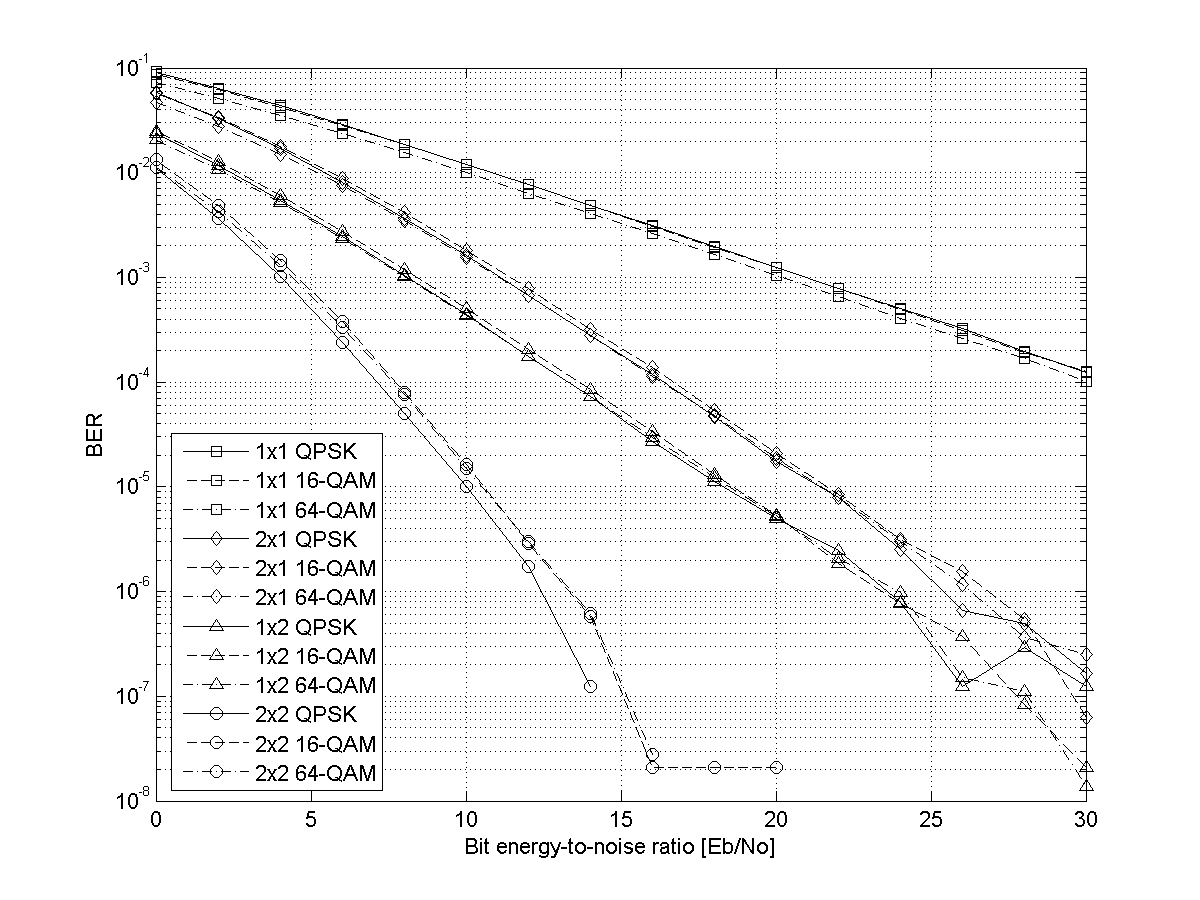
\includegraphics[width=0.8\textwidth]{images/result1.png}
  \caption{Comparison of BER versus $E_b/N_0$ for small MIMO and stationary receiver.}
  \label{fig:result1}
\end{figure}

\begin{figure}[p]
  \centering
  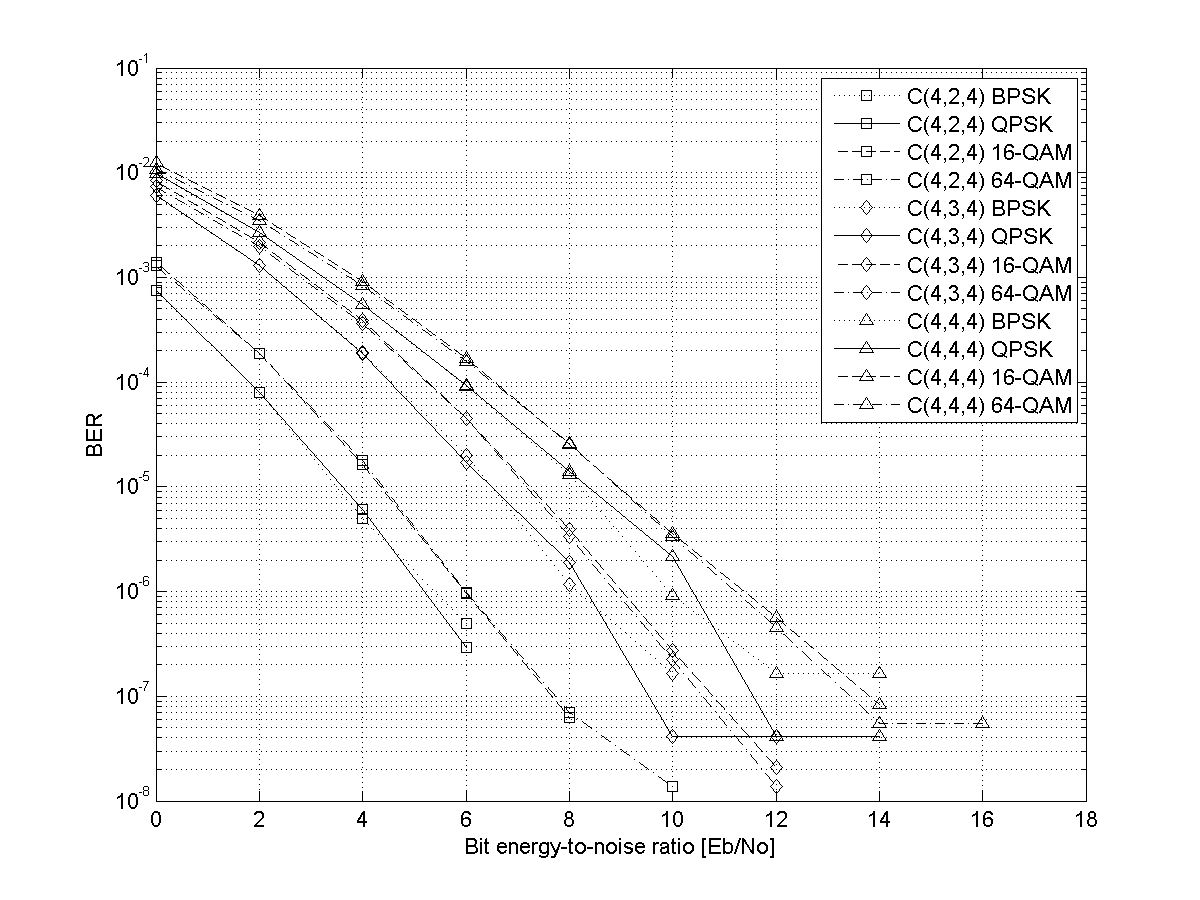
\includegraphics[width=0.8\textwidth]{images/result2.png}
  \caption{Comparison of BER versus $E_b/N_0$ for $N_T=4$ and stationary receiver.}
  \label{fig:result2}
\end{figure}

\begin{figure}[p]
  \centering
  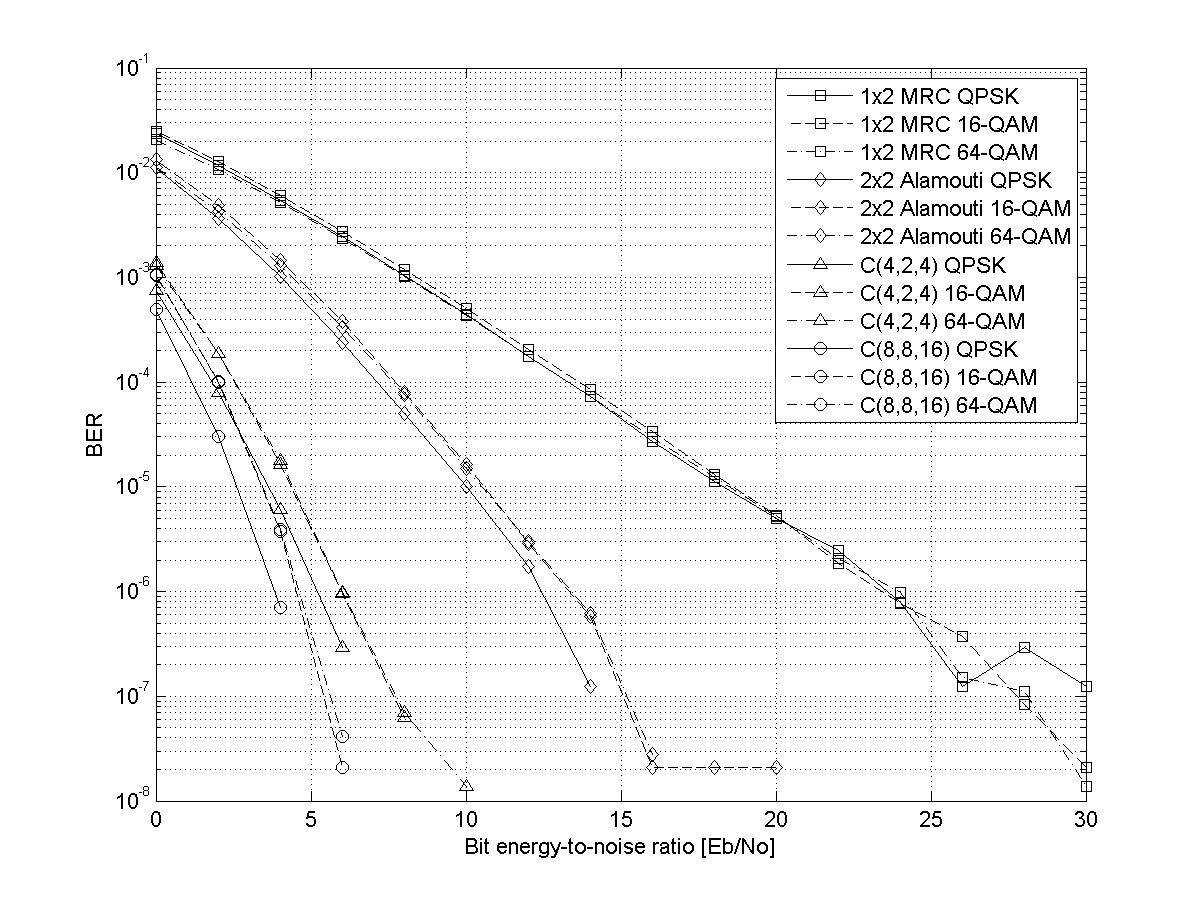
\includegraphics[width=0.8\textwidth]{images/result3.png}
  \caption{Comparison of BER versus $E_b/N_0$ for various $N_T$ and stationary receiver.}
  \label{fig:result3}
\end{figure}

\begin{figure}[p]
  \centering
  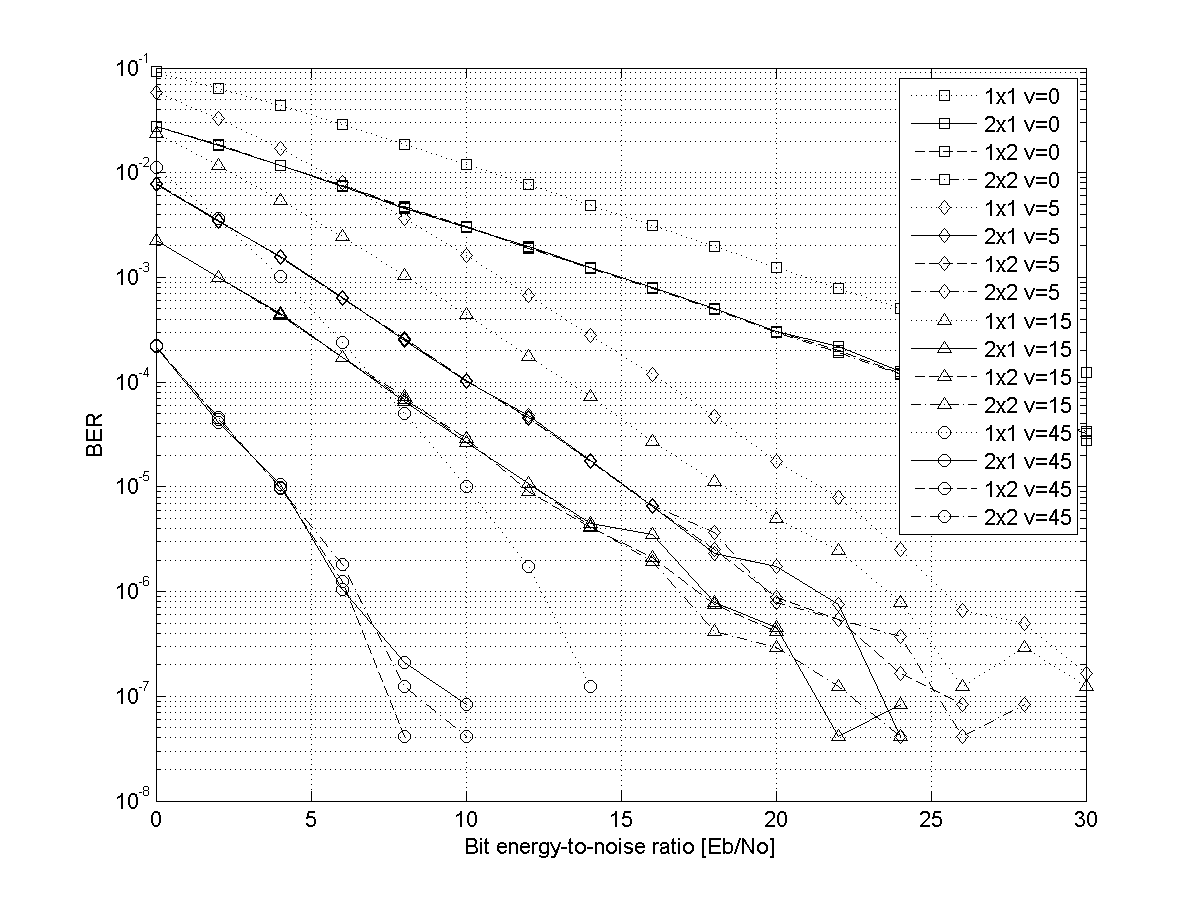
\includegraphics[width=0.8\textwidth]{images/result4a.png}
  \caption{Comparison of BER versus $E_b/N_0$ for QPSK, small MIMO, and moving receiver.}
  \label{fig:result4a}
\end{figure}

\begin{figure}[p]
  \centering
  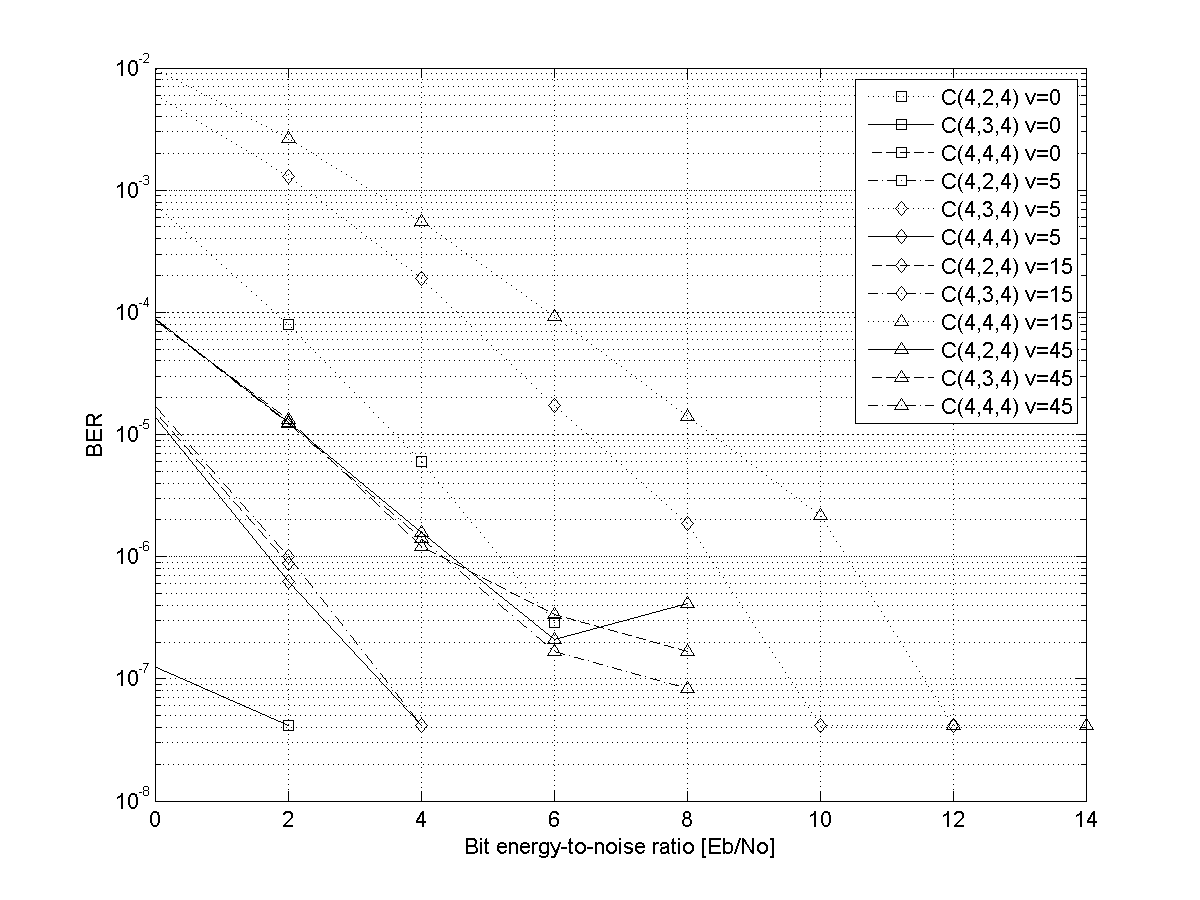
\includegraphics[width=0.8\textwidth]{images/result4b.png}
  \caption{Comparison of BER versus $E_b/N_0$ for QPSK, $N_T=4$, and moving receiver.}
  \label{fig:result4b}
\end{figure}

\begin{figure}[p]
  \centering
  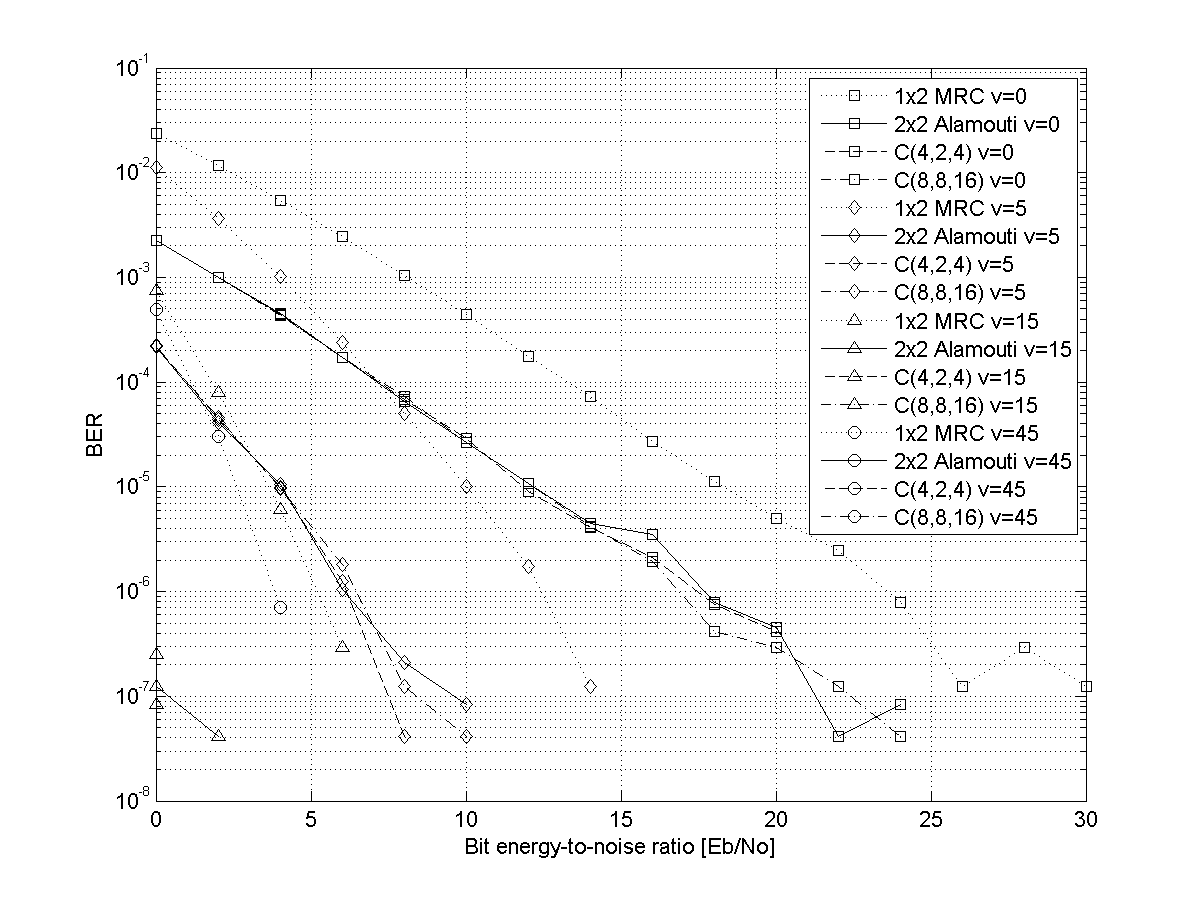
\includegraphics[width=0.8\textwidth]{images/result5.png}
  \caption{Comparison of BER versus $E_b/N_0$ for QPSK, various $N_T$, and moving receiver.}
  \label{fig:result5}
\end{figure}

\section{Summary}
%%% Local Variables:
%%% mode: latex
%%% TeX-master: "report"
%%% End:

% Section VI: Summary

This paper compared the performance of various STBC schemes for a flat Rayleigh block-fading channel with AWGN. The simulation results showed that the $C(4,2,4)$ coded had the best tradeoff between implementation simplicity, performance, and spectral efficiency. Additionally, for the particular channel considered by this paper, increasing the speed of the receiver actually increased performance. The authors believe that this is due to the use of MRC at the decoder. This special channel case is likely not realistic so future investigations should consider a more realistic channel.

Extending these results to future 5G technologies, likely using massive MIMO, the authors believe that rate $R=1/2$ OSTBC schemes should be considered. While having a lower rate than QOSTBC schemes as well as MRC with $N_T=1$, for a given BER it was consistently more than 3~dB better than an equivalent diversity code with higher rate. Additionally, the linearity of these codes and the ease of generation using HR families is beneficial for design and use of these codes.

\bibliography{report}

\appendix

The appendix is organized as follows. The first two sections contain functions for simulating the STBC-MIMO channel for the eight STBCs and any given modulation and demodulation methods. The code in the rest of the sections implement encoding and decoding of the various STBCs. The following sample script shows how to perform a simulation run.

\begin{lstlisting}
%% simulation parameters
numPackets = 1e5; % each packets contains 120 symbols
EbNo = 0:2:30; % in dB
v = 5; % speed for calculating Doppler frequency in m/s

%% calculate normalized Doppler frequency
Ts = 1/15e3; % symbol rate is 15 kHz = sub-carrier spacing for LTE
fc = 1800e6; % carrier freq of 1800 MHz
fm_norm = v*fc/3e8*Ts; % normalized max. Doppler freq. (fm*Ts)

%% modulation method
% 16-QAM shown
M = 16;
hMod = comm.RectangularQAMModulator(M, ...
    'NormalizationMethod', 'Average power', 'BitInput', true);
hDemod = comm.RectangularQAMDemodulator(M, ...
    'NormalizationMethod', 'Average power', 'BitOutput', true);
% uncomment below lines for PSK
% hMod = comm.PSKModulator(M, 'PhaseOffset', 0, ...
%     'BitInput', true);
% hDemod = comm.PSKDemodulator(M, 'PhaseOffset', 0, ...
%     'BitOutput', true);

%% Run simulation
% stationary MS
% ber = sim_flatRayleigh(EbNo,numPackets,M,hMod,hDemod);
% moving MS
ber = sim_flatRayleighDoppler(EbNo,numPackets,M,hMod,hDemod, ...
    fm_norm);
\end{lstlisting}

\appendices

\section{Stationary Receiver}
\lstinputlisting{code/sim_flatRayleigh.m}
\section{Mobile Receiver}
\lstinputlisting{code/sim_flatRayleighDoppler.m}
\section{MRC: $1\times2$}
\lstinputlisting{code/fun_MRCx2.m}
\section{Alamouti Encoding}
\lstinputlisting{code/fun_AlamoutiEnc.m}
\section{Alamouti Decoding: $2\times1$}
\lstinputlisting{code/fun_AlamoutiDec2x1.m}
\section{Alamouti Decoding: $2\times2$}
\lstinputlisting{code/fun_AlamoutiDec2x2.m}
\section{$C(4,4,8)$ Encoding}
\lstinputlisting{code/fun_OSTBC2Enc4x.m}
\section{$C(4,4,8)$ Decoding: $4\times2$}
\lstinputlisting{code/fun_OSTBC2Dec4x2.m}
\section{$C(4,3,4)$ Encoding}
\lstinputlisting{code/fun_OSTBCEnc4x.m}
\section{$C(4,3,4)$ Decoding: $4\times2$}
\lstinputlisting{code/fun_OSTBCDec4x2.m}
\section{$C(4,4,4)$ Encoding}
\lstinputlisting{code/fun_QOSTBCEnc4x.m}
\section{$C(4,4,4)$ Decoding: $4\times2$}
\lstinputlisting{code/fun_QOSTBCDec4x2.m}
\section{$C(8,8,16)$ Encoding}
\lstinputlisting{code/fun_OSTBC2Enc4x.m}
\section{$C(8,8,16)$ Decoding: $8\times2$}
\lstinputlisting{code/fun_OSTBC2Dec4x2.m}

\end{document}
